\documentclass[twoside]{book}

% Packages required by doxygen
\usepackage{calc}
\usepackage{doxygen}
\usepackage{graphicx}
\usepackage[utf8]{inputenc}
\usepackage{makeidx}
\usepackage{multicol}
\usepackage{multirow}
\usepackage{textcomp}
\usepackage[table]{xcolor}

% Font selection
\usepackage[T1]{fontenc}
\usepackage{mathptmx}
\usepackage[scaled=.90]{helvet}
\usepackage{courier}
\usepackage{amssymb}
\usepackage{sectsty}
\renewcommand{\familydefault}{\sfdefault}
\allsectionsfont{%
  \fontseries{bc}\selectfont%
  \color{darkgray}%
}
\renewcommand{\DoxyLabelFont}{%
  \fontseries{bc}\selectfont%
  \color{darkgray}%
}

% Page & text layout
\usepackage{geometry}
\geometry{%
  a4paper,%
  top=2.5cm,%
  bottom=2.5cm,%
  left=2.5cm,%
  right=2.5cm%
}
\tolerance=750
\hfuzz=15pt
\hbadness=750
\setlength{\emergencystretch}{15pt}
\setlength{\parindent}{0cm}
\setlength{\parskip}{0.2cm}
\makeatletter
\renewcommand{\paragraph}{%
  \@startsection{paragraph}{4}{0ex}{-1.0ex}{1.0ex}{%
    \normalfont\normalsize\bfseries\SS@parafont%
  }%
}
\renewcommand{\subparagraph}{%
  \@startsection{subparagraph}{5}{0ex}{-1.0ex}{1.0ex}{%
    \normalfont\normalsize\bfseries\SS@subparafont%
  }%
}
\makeatother

% Headers & footers
\usepackage{fancyhdr}
\pagestyle{fancyplain}
\fancyhead[LE]{\fancyplain{}{\bfseries\thepage}}
\fancyhead[CE]{\fancyplain{}{}}
\fancyhead[RE]{\fancyplain{}{\bfseries\leftmark}}
\fancyhead[LO]{\fancyplain{}{\bfseries\rightmark}}
\fancyhead[CO]{\fancyplain{}{}}
\fancyhead[RO]{\fancyplain{}{\bfseries\thepage}}
\fancyfoot[LE]{\fancyplain{}{}}
\fancyfoot[CE]{\fancyplain{}{}}
\fancyfoot[RE]{\fancyplain{}{\bfseries\scriptsize Generated on Fri Jul 27 2018 10\-:23\-:35 for Continous\-Integration\-Playground by Doxygen }}
\fancyfoot[LO]{\fancyplain{}{\bfseries\scriptsize Generated on Fri Jul 27 2018 10\-:23\-:35 for Continous\-Integration\-Playground by Doxygen }}
\fancyfoot[CO]{\fancyplain{}{}}
\fancyfoot[RO]{\fancyplain{}{}}
\renewcommand{\footrulewidth}{0.4pt}
\renewcommand{\chaptermark}[1]{%
  \markboth{#1}{}%
}
\renewcommand{\sectionmark}[1]{%
  \markright{\thesection\ #1}%
}

% Indices & bibliography
\usepackage{natbib}
\usepackage[titles]{tocloft}
\setcounter{tocdepth}{3}
\setcounter{secnumdepth}{5}
\makeindex

% Hyperlinks (required, but should be loaded last)
\usepackage{ifpdf}
\ifpdf
  \usepackage[pdftex,pagebackref=true]{hyperref}
\else
  \usepackage[ps2pdf,pagebackref=true]{hyperref}
\fi
\hypersetup{%
  colorlinks=true,%
  linkcolor=blue,%
  citecolor=blue,%
  unicode%
}

% Custom commands
\newcommand{\clearemptydoublepage}{%
  \newpage{\pagestyle{empty}\cleardoublepage}%
}


%===== C O N T E N T S =====

\begin{document}

% Titlepage & ToC
\hypersetup{pageanchor=false}
\pagenumbering{roman}
\begin{titlepage}
\vspace*{7cm}
\begin{center}%
{\Large Continous\-Integration\-Playground }\\
\vspace*{1cm}
{\large Generated by Doxygen 1.8.6}\\
\vspace*{0.5cm}
{\small Fri Jul 27 2018 10:23:35}\\
\end{center}
\end{titlepage}
\clearemptydoublepage
\tableofcontents
\clearemptydoublepage
\pagenumbering{arabic}
\hypersetup{pageanchor=true}

%--- Begin generated contents ---
\chapter{Continous Integration Playground}
\label{md__home_travis_build__m_r_konrad__continous_integration_playground__r_e_a_d_m_e}
\hypertarget{md__home_travis_build__m_r_konrad__continous_integration_playground__r_e_a_d_m_e}{}
See the \href{https://mrkonrad.github.io/ContinousIntegrationPlayground/}{\tt D\-O\-C\-S P\-A\-G\-E}

\begin{TabularC}{2}
\hline
\rowcolor{lightgray}\PBS\centering {\bf System }&\PBS\centering {\bf Status  }\\\cline{1-2}
\PBS\centering Travis (O\-S\-X/\-Linux) &\PBS\centering \href{https://travis-ci.org/MRKonrad/ContinousIntegrationPlayground}{\tt !\mbox{[}Travis (.org)\mbox{]}(https\-://img.\-shields.\-io/travis/\-M\-R\-Konrad/\-Continous\-Integration\-Playground.\-svg?style=for-\/the-\/badge)} \\\cline{1-2}
\PBS\centering App\-Veyor (Windows) &\PBS\centering \href{https://ci.appveyor.com/project/MRKonrad/continousintegrationplayground}{\tt !\mbox{[}App\-Veyor\mbox{]}(https\-://img.\-shields.\-io/appveyor/ci/\-M\-R\-Konrad/continousintegrationplayground.\-svg?style=for-\/the-\/badge)} \\\cline{1-2}
\PBS\centering Coveralls (test coverage) &\PBS\centering \href{https://coveralls.io/github/MRKonrad/ContinousIntegrationPlayground}{\tt !\mbox{[}Coveralls\mbox{]}(https\-://img.\-shields.\-io/coveralls/github/\-M\-R\-Konrad/\-Continous\-Integration\-Playground.\-svg?style=for-\/the-\/badge)} \\\cline{1-2}
\end{TabularC}


\section*{Inspiration}

Based on
\begin{DoxyItemize}
\item \href{https://github.com/LearningByExample/ModernCppCI}{\tt this repo}
\item \href{http://david-grs.github.io/cpp-clang-travis-cmake-gtest-coveralls-appveyor/}{\tt this post} about travis, cmake, gtest, coveralls and appveyor
\item \href{https://gist.github.com/vidavidorra/7ed6166a46c537d3cbd2}{\tt this gist} about doxygen, travis and github
\end{DoxyItemize}

\section*{Notes}


\begin{DoxyItemize}
\item entries in {\ttfamily .gitmodules} are added automatically by calling for example {\ttfamily git submodule add \href{https://github.com/google/googletest.git}{\tt https\-://github.\-com/google/googletest.\-git} ./third\-Party/googletest}
\item to generate coverage {\ttfamily lcov -\/-\/capture -\/-\/directory . -\/-\/output-\/file coverage.\-info}
\item to generate coverage html report {\ttfamily genhtml coverage.\-info -\/-\/output-\/directory out} 
\end{DoxyItemize}
\chapter{File Index}
\section{File List}
Here is a list of all documented files with brief descriptions\-:\begin{DoxyCompactList}
\item\contentsline{section}{/home/travis/build/\-M\-R\-Konrad/\-Continous\-Integration\-Playground/\hyperlink{mylib_8h}{mylib.\-h} \\*A Documented file }{\pageref{mylib_8h}}{}
\end{DoxyCompactList}

\chapter{File Documentation}
\hypertarget{main_8cpp}{\section{/home/travis/build/\-M\-R\-Konrad/\-Continous\-Integration\-Playground/app/main.cpp File Reference}
\label{main_8cpp}\index{/home/travis/build/\-M\-R\-Konrad/\-Continous\-Integration\-Playground/app/main.\-cpp@{/home/travis/build/\-M\-R\-Konrad/\-Continous\-Integration\-Playground/app/main.\-cpp}}
}


A Documented file with main.  


{\ttfamily \#include $<$iostream$>$}\\*
{\ttfamily \#include \char`\"{}mylib.\-h\char`\"{}}\\*
Include dependency graph for main.\-cpp\-:
\nopagebreak
\begin{figure}[H]
\begin{center}
\leavevmode
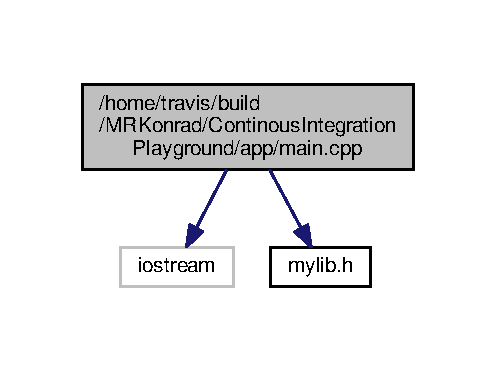
\includegraphics[width=238pt]{main_8cpp__incl}
\end{center}
\end{figure}
\subsection*{Functions}
\begin{DoxyCompactItemize}
\item 
int \hyperlink{main_8cpp_ae66f6b31b5ad750f1fe042a706a4e3d4}{main} ()
\end{DoxyCompactItemize}


\subsection{Detailed Description}
A Documented file with main. Details of the file should be here. L\-O\-L \begin{DoxyAuthor}{Author}
Konrad Werys 
\end{DoxyAuthor}
\begin{DoxyDate}{Date}
2018/08/24 
\end{DoxyDate}


\subsection{Function Documentation}
\hypertarget{main_8cpp_ae66f6b31b5ad750f1fe042a706a4e3d4}{\index{main.\-cpp@{main.\-cpp}!main@{main}}
\index{main@{main}!main.cpp@{main.\-cpp}}
\subsubsection[{main}]{\setlength{\rightskip}{0pt plus 5cm}int main (
\begin{DoxyParamCaption}
{}
\end{DoxyParamCaption}
)}}\label{main_8cpp_ae66f6b31b5ad750f1fe042a706a4e3d4}
main \begin{DoxyReturn}{Returns}
always 0 
\end{DoxyReturn}

\hypertarget{mylib_8h}{\section{/home/travis/build/\-M\-R\-Konrad/\-Continous\-Integration\-Playground/lib/mylib.h File Reference}
\label{mylib_8h}\index{/home/travis/build/\-M\-R\-Konrad/\-Continous\-Integration\-Playground/lib/mylib.\-h@{/home/travis/build/\-M\-R\-Konrad/\-Continous\-Integration\-Playground/lib/mylib.\-h}}
}


A Documented file.  


This graph shows which files directly or indirectly include this file\-:
\nopagebreak
\begin{figure}[H]
\begin{center}
\leavevmode
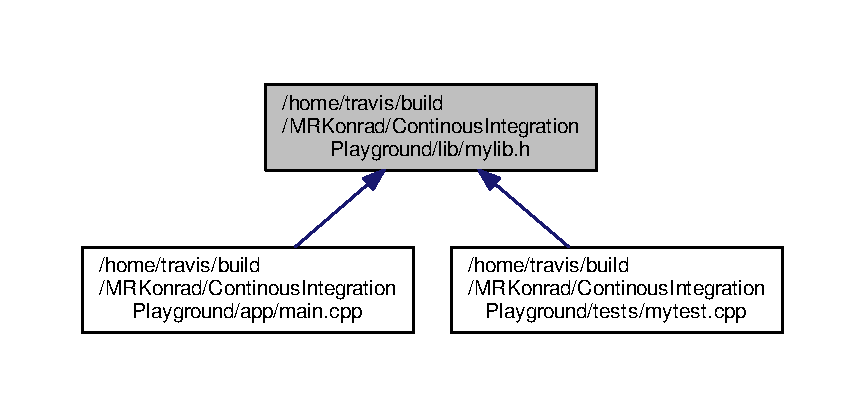
\includegraphics[width=350pt]{mylib_8h__dep__incl}
\end{center}
\end{figure}
\subsection*{Functions}
\begin{DoxyCompactItemize}
\item 
int \hyperlink{mylib_8h_af79a6d67c4a1b0b4f744da2f5bb780f4}{dummy\-Function} (int input)
\begin{DoxyCompactList}\small\item\em a dummy function that returns the output integer \end{DoxyCompactList}\end{DoxyCompactItemize}


\subsection{Detailed Description}
A Documented file. Details of the file should be here. L\-O\-L \begin{DoxyAuthor}{Author}
Konrad Werys 
\end{DoxyAuthor}
\begin{DoxyDate}{Date}
2018/08/24 
\end{DoxyDate}


\subsection{Function Documentation}
\hypertarget{mylib_8h_af79a6d67c4a1b0b4f744da2f5bb780f4}{\index{mylib.\-h@{mylib.\-h}!dummy\-Function@{dummy\-Function}}
\index{dummy\-Function@{dummy\-Function}!mylib.h@{mylib.\-h}}
\subsubsection[{dummy\-Function}]{\setlength{\rightskip}{0pt plus 5cm}int dummy\-Function (
\begin{DoxyParamCaption}
\item[{int}]{input}
\end{DoxyParamCaption}
)}}\label{mylib_8h_af79a6d67c4a1b0b4f744da2f5bb780f4}


a dummy function that returns the output integer 


\begin{DoxyParams}{Parameters}
{\em input} & \\
\hline
\end{DoxyParams}
\begin{DoxyReturn}{Returns}
input 
\end{DoxyReturn}

\hypertarget{mylib2_8h}{\section{/home/travis/build/\-M\-R\-Konrad/\-Continous\-Integration\-Playground/lib/mylib2.h File Reference}
\label{mylib2_8h}\index{/home/travis/build/\-M\-R\-Konrad/\-Continous\-Integration\-Playground/lib/mylib2.\-h@{/home/travis/build/\-M\-R\-Konrad/\-Continous\-Integration\-Playground/lib/mylib2.\-h}}
}


A Documented file.  


\subsection*{Functions}
\begin{DoxyCompactItemize}
\item 
int \hyperlink{mylib2_8h_a62d4f526974e27175a3bfe6d8be46598}{dummy\-Function2} (int input)
\begin{DoxyCompactList}\small\item\em a dummy function that returns the output integer \end{DoxyCompactList}\end{DoxyCompactItemize}


\subsection{Detailed Description}
A Documented file. Details of the file should be here. L\-O\-L \begin{DoxyAuthor}{Author}
Konrad Werys 
\end{DoxyAuthor}
\begin{DoxyDate}{Date}
2018/08/24 
\end{DoxyDate}


\subsection{Function Documentation}
\hypertarget{mylib2_8h_a62d4f526974e27175a3bfe6d8be46598}{\index{mylib2.\-h@{mylib2.\-h}!dummy\-Function2@{dummy\-Function2}}
\index{dummy\-Function2@{dummy\-Function2}!mylib2.h@{mylib2.\-h}}
\subsubsection[{dummy\-Function2}]{\setlength{\rightskip}{0pt plus 5cm}int dummy\-Function2 (
\begin{DoxyParamCaption}
\item[{int}]{input}
\end{DoxyParamCaption}
)}}\label{mylib2_8h_a62d4f526974e27175a3bfe6d8be46598}


a dummy function that returns the output integer 


\begin{DoxyParams}{Parameters}
{\em input} & \\
\hline
\end{DoxyParams}
\begin{DoxyReturn}{Returns}
input 
\end{DoxyReturn}

\hypertarget{mylib3_8h}{\section{/home/travis/build/\-M\-R\-Konrad/\-Continous\-Integration\-Playground/lib/mylib3.h File Reference}
\label{mylib3_8h}\index{/home/travis/build/\-M\-R\-Konrad/\-Continous\-Integration\-Playground/lib/mylib3.\-h@{/home/travis/build/\-M\-R\-Konrad/\-Continous\-Integration\-Playground/lib/mylib3.\-h}}
}


A Documented file.  


\subsection*{Functions}
\begin{DoxyCompactItemize}
\item 
int \hyperlink{mylib3_8h_ae34c1132a2ea658adbdb0f3042e13d51}{dummy\-Function3} (int input)
\begin{DoxyCompactList}\small\item\em a dummy function that returns the output integer \end{DoxyCompactList}\end{DoxyCompactItemize}


\subsection{Detailed Description}
A Documented file. Details of the file should be here. L\-O\-L \begin{DoxyAuthor}{Author}
Konrad Werys 
\end{DoxyAuthor}
\begin{DoxyDate}{Date}
2018/08/24 
\end{DoxyDate}


\subsection{Function Documentation}
\hypertarget{mylib3_8h_ae34c1132a2ea658adbdb0f3042e13d51}{\index{mylib3.\-h@{mylib3.\-h}!dummy\-Function3@{dummy\-Function3}}
\index{dummy\-Function3@{dummy\-Function3}!mylib3.h@{mylib3.\-h}}
\subsubsection[{dummy\-Function3}]{\setlength{\rightskip}{0pt plus 5cm}int dummy\-Function3 (
\begin{DoxyParamCaption}
\item[{int}]{input}
\end{DoxyParamCaption}
)}}\label{mylib3_8h_ae34c1132a2ea658adbdb0f3042e13d51}


a dummy function that returns the output integer 


\begin{DoxyParams}{Parameters}
{\em input} & \\
\hline
\end{DoxyParams}
\begin{DoxyReturn}{Returns}
input 
\end{DoxyReturn}

\hypertarget{mytest_8cpp}{\section{/home/travis/build/\-M\-R\-Konrad/\-Continous\-Integration\-Playground/tests/mytest.cpp File Reference}
\label{mytest_8cpp}\index{/home/travis/build/\-M\-R\-Konrad/\-Continous\-Integration\-Playground/tests/mytest.\-cpp@{/home/travis/build/\-M\-R\-Konrad/\-Continous\-Integration\-Playground/tests/mytest.\-cpp}}
}


A Documented test file.  


{\ttfamily \#include \char`\"{}gtest/gtest.\-h\char`\"{}}\\*
{\ttfamily \#include \char`\"{}mylib.\-h\char`\"{}}\\*
Include dependency graph for mytest.\-cpp\-:
\nopagebreak
\begin{figure}[H]
\begin{center}
\leavevmode
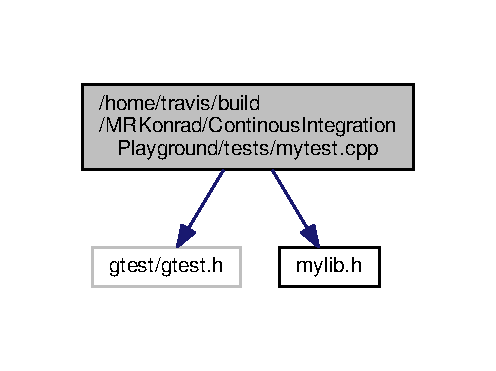
\includegraphics[width=238pt]{mytest_8cpp__incl}
\end{center}
\end{figure}
\subsection*{Functions}
\begin{DoxyCompactItemize}
\item 
\hyperlink{mytest_8cpp_a5318fbaff420e483239371af8e6df235}{T\-E\-S\-T} (Continous\-Integration\-Playground, Dummy\-Test)
\item 
\hyperlink{mytest_8cpp_a05b1b372df5d685b6e0a75fc88628ba3}{T\-E\-S\-T} (Continous\-Integration\-Playground, Dummy\-Function\-Test)
\end{DoxyCompactItemize}


\subsection{Detailed Description}
A Documented test file. Details of the file should be here. L\-O\-L \begin{DoxyAuthor}{Author}
Konrad Werys 
\end{DoxyAuthor}
\begin{DoxyDate}{Date}
2018/08/24 
\end{DoxyDate}


\subsection{Function Documentation}
\hypertarget{mytest_8cpp_a5318fbaff420e483239371af8e6df235}{\index{mytest.\-cpp@{mytest.\-cpp}!T\-E\-S\-T@{T\-E\-S\-T}}
\index{T\-E\-S\-T@{T\-E\-S\-T}!mytest.cpp@{mytest.\-cpp}}
\subsubsection[{T\-E\-S\-T}]{\setlength{\rightskip}{0pt plus 5cm}T\-E\-S\-T (
\begin{DoxyParamCaption}
\item[{Continous\-Integration\-Playground}]{, }
\item[{Dummy\-Test}]{}
\end{DoxyParamCaption}
)}}\label{mytest_8cpp_a5318fbaff420e483239371af8e6df235}
Dummy test compares 1 with 1 \hypertarget{mytest_8cpp_a05b1b372df5d685b6e0a75fc88628ba3}{\index{mytest.\-cpp@{mytest.\-cpp}!T\-E\-S\-T@{T\-E\-S\-T}}
\index{T\-E\-S\-T@{T\-E\-S\-T}!mytest.cpp@{mytest.\-cpp}}
\subsubsection[{T\-E\-S\-T}]{\setlength{\rightskip}{0pt plus 5cm}T\-E\-S\-T (
\begin{DoxyParamCaption}
\item[{Continous\-Integration\-Playground}]{, }
\item[{Dummy\-Function\-Test}]{}
\end{DoxyParamCaption}
)}}\label{mytest_8cpp_a05b1b372df5d685b6e0a75fc88628ba3}
Dummy test of a dummy\-Function 
%--- End generated contents ---

% Index
\newpage
\phantomsection
\addcontentsline{toc}{chapter}{Index}
\printindex

\end{document}
